\newpage
\section*{Problem 6:}
We used our implementation of Lanczos-based approach and run it on the data of \texttt{FP\_Ex2.mat}. Figure~\ref{fig:fig2} shows the results with $s0 = 10^{10}$ and $k = 1000$.  Function \texttt{Figure\_2()} in \texttt{driver.m} file generates this plot. 

\begin{figure}[!tbh]
\centering        
   \subfloat {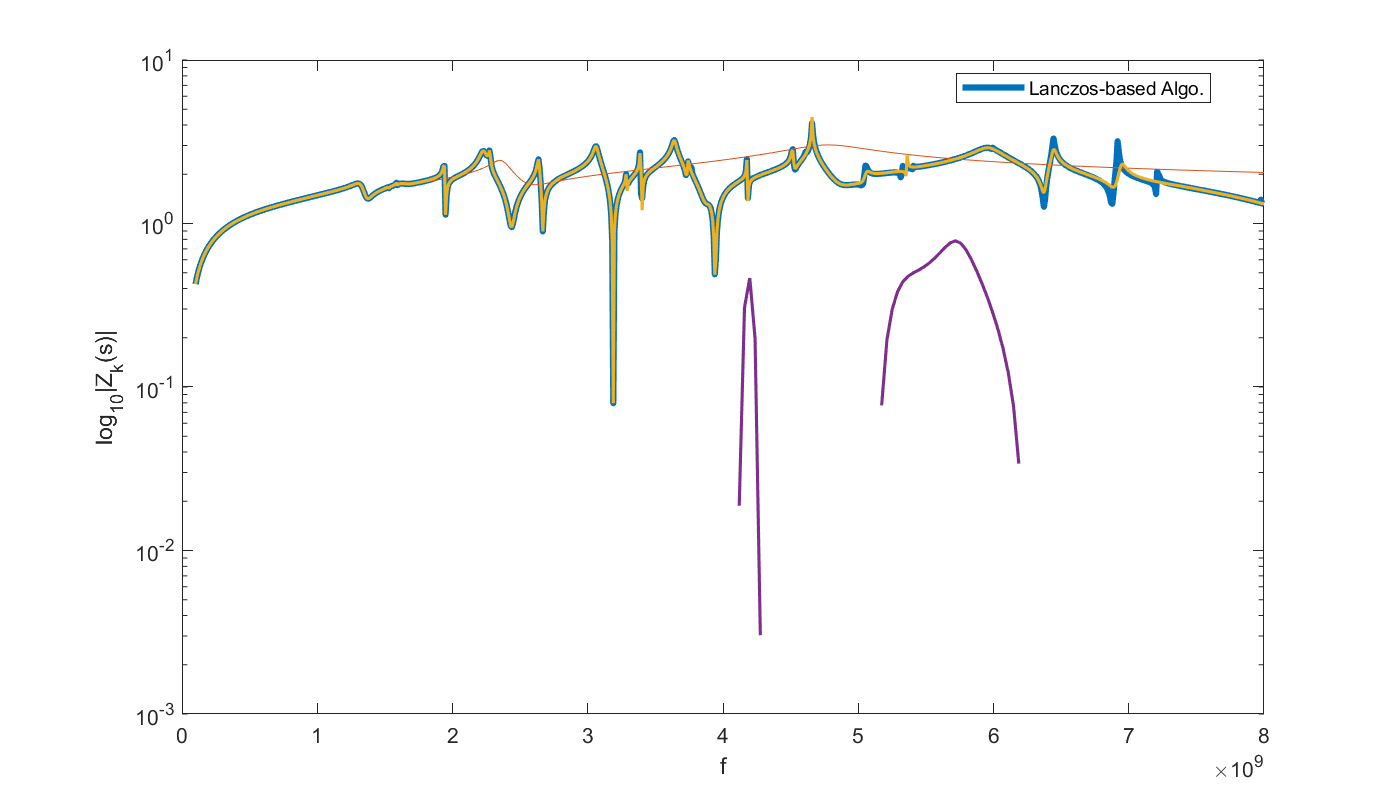
\includegraphics[width=0.85\textwidth]{../code/figure2.png}}
   \caption{Results of the Lanczos-based approach on Example 2 input with $s0 = 10^{10}$ and $k = 1000$ }
   \label{fig:fig2}
\end{figure}

\paragraph{Lanczos approach with difference $s_{0}$:}  We runs similar test as we did in previous problem to see the effect of $s_{0}$. Since the problem is more expensive to solve, we run $k$ in a loop that increment by 100 between 200 and 10000. We choose similar $s_{0}$ as we did before and the results is shown in Table~\ref{tab:s02}. In addition, we reduce the tolerance to 10^{-3}. The tolerance here means the norm squared of difference between results of $Z_{k}(s)$ and $Z_{k-1}(s)$. We can observe similar behaviour similar to what we have seen in previous example; while complex $s_{0}$ give good approximation at smaller $k$, they are more expensive to evaluate. In addition, extreme cases with complex component that is equal to $f_{min}$ is actually better than this that is equal to $f_{max}$. Real $s_{0}$ could be very costly because it needs to run for much larger $k$ values. 


\begin{table}[!tbh]
 \centering    
\begin{tabular}{ ||p{3.0cm}|p{1.5cm}| p{4cm}| p{4cm}||}
\hline
 $s_{0}$  & $k$ & Time & Average Difference \\ \hhline{|=|=|=|=|} 
 $10^{10} + 2 \pi i f_{avg}$ & 600 & $\expnumber{1.420857}{2}$ & $\expnumber{2.174922}{-4}$ \\
 $10^{10} + 2 \pi i f_{min}$ & 700 & $\expnumber{1.673579}{2}$ & $\expnumber{3.999830}{-4}$ \\
 $10^{10} + 2 \pi i f_{max}$ & 1500& $\expnumber{4.133558}{2}$& $\expnumber{1.401831}{-4}$\\
 $10^{8} $                   &  4000   & $\expnumber{ 1.50910687370000}{3}$& $\expnumber{1.308395158595435}{-3}$ \\
 $10^{12}$                   & 2100 & $\expnumber{5.529143}{2}$& $\expnumber{1.235801}{-4}$\\  
\hline
\end{tabular} 
\caption{Experimenting with Lanczos approach using different $s_{0}$ values ($f_{avg} = \frac{f_{min}+f_{max}}{2}$) }
   \label{tab:s02}
\end{table}